%% LyX 2.3.1-1 created this file.  For more info, see http://www.lyx.org/.
%% Do not edit unless you really know what you are doing.
\documentclass[11pt,english]{article}
\usepackage{ae,aecompl}
\usepackage[T1]{fontenc}
\usepackage[latin9]{inputenc}
\usepackage[letterpaper]{geometry}
\geometry{verbose,tmargin=2.54cm,bmargin=2.54cm}
\setcounter{secnumdepth}{4}
\usepackage{amsmath}
\usepackage{graphicx}
\usepackage[numbers]{natbib}

\makeatletter
%%%%%%%%%%%%%%%%%%%%%%%%%%%%%% User specified LaTeX commands.
\usepackage{graphicx}
\usepackage{pdflscape}
%\usepackage[cm]{fullpage}
%\usepackage[compact]{titlesec}
%\date{}
\usepackage{scicite}

\makeatother

\usepackage{babel}
\begin{document}
\title{Supplementary Materials}
\author{Mohammed Chamma}
\maketitle

\section*{Materials and Methods}

This section will describe the process of deriving measurements of
the sub-burst drift rate and the burst duration from dynamic spectra
of Fast Radio Bursts, and is largely based on the autocorrelation
technique described in \cite{Hessels2019,CHIME2019c}. In addition,
we describe tests to the robustness of the inverse trend between the
drift rate and the burst duration through variations of the DM, which
show that small variations of the DM serve to rotate the FRB dynamic
spectra, and, even though they affect the measured value of the sub-burst
drift rate, do not affect the relative trend between bursts.

Dynamic spectra of bursts are obtained from several sources and processed
based on the format they are made available in, and are typically
dedispersed to the DMs presented in their respective publications.
Bursts from the repeater FRB121102 were obtained from \cite{Gajjar2018,Michilli2018,CHIME2019c}.
These data were taken as presented in Fig. 2 of \cite{Gajjar2018},
Fig. 1 of \cite{Michilli2018}, and Fig. 5 of \cite{CHIME2019c},
and range in frequency from \textasciitilde 600 Mhz to 8 GHz. For
all bursts from FRB121102, we used the structure-optimized dedispersed
spectra without modification which corresponds to DMs of 565, 559.7,
and 563.6 pc/cm$^{3}$ from \cite{Gajjar2018,Michilli2018,CHIME2019c},
respectively. Data for FRB180916.J0158+65 and FRB180814.J0422+73 are
available from the public data archive for the CHIME telescope (chime-frb-open-data.github.io)
\cite{CHIME2019a,Amiri2020periodic}. Dedispersed bursts from FRB180916.J0158+65
are used at a DM of 348.82 pc/cm$^{3}$, though we also investigated
the effect of small variations of this DM, as discussed later. Data
for FRB180814.J0422+74 is provided at its original resolution and
without dedispersion. The range of DMs used for this source in \cite{CHIME2019a}
vary between 188.9-190 pc/cm$^{3}$. We find that a good fit between
this data and our model exists for DMs in between 188.9-189.4 pc/cm$^{3}$.
However we will tentatively argue that the shape of the FRB180814.J0422+7
bursts suggests too aggressive of a dedispersion and that a slightly
lower DM of 188.7-188.8 pc/cm$^{3}$ is optimal in terms of the burst
shape expected when taken in context with the bursts from the other
two sources. In all cases dynamic spectra are downsampled in frequency
to increase SNR. When a dynamic spectrum consists of a train of multiple
bursts, we separate the components and measure the drift rate and
duration of each burst separately, as described in Fig 3. of \cite{Rajabi2020b}.

Even when from the same source, fast radio bursts can have DMs that
differ from each other and that potentially also vary with time \cite{Gajjar2018},
which raises questions about which DM is appropriate to use. For this
work we choose a single DM per source since multiple bursts from short
duration pulse trains (which should have a single canonical DM) obey
the inverse relationship between the sub-burst drift rate and burst
duration, and a single DM simplifies the analysis. We found that small
variations in the DM (on the order of 5\%) can increase the spread
of the points on a drift vs. duration plot and can translate the points
up or down, which clearly affects the fit, but the existence of the
relationship in general remains. Additionally, because the DM is primarily
a property of the interstellar medium and not the source, any model
that requires a fine-tuned selection of DMs adds additional parameters
and complexity that require justification. For example, a model that
selects DMs based on maximizing structure \cite{Gajjar2018,Hessels2019}
as a selection criteria brings with it assumptions that components
of the burst are emitted (and arrive) simultaneously across a large
frequency range \cite{Hessels2019}. While this criteria advantageously
gives a narrow range of DMs to choose from, there is no reason to
strictly adhere to it from burst to burst. Therefore, in general,
we limit ourselves to the range of DMs found from all the bursts as
a whole when considering variations, and for the analysis proper we
select a single DM for every burst from a particular source.

The general pipeline that every burst is put through is written in
Python and consists of computing the autocorrelation of the signal,
fitting a two-dimensional Gaussian to the resulting autocorrelation,
and a calculation of the physical quantities of interest from the
fit parameters: namely the sub-burst drift rate and the burst duration.
The autocorrelation of the spectrum measures the self-similarity of
the burst in frequency and time space and for FRBs results in an ellipsoid
with an intensity that follows a 2D Gaussian \cite{Hessels2019}.
Before autocorrelation and depending on the source and/or burst, some
noise removal is performed. For the bursts from FRB121102 and FRB180916.J0158+65
this is done by subtracting the background from the entire spectrum,
which is obtained from a time-average of twenty or so samples taken
prior to the burst. For FRB180814.J0422+73, due to the raw format
the bursts are provided in, a noise mask was acquired through correspondence
and the channels are normalized by the standard deviation of the intensity.
We compute the autocorrelation of the dynamic spectrum using an intermediate
FFT, which allows us to perform the correlation through a multiplication
and is much faster. After multiplication we perform an inverse FFT
and the result is the autocorrelation of the burst. The shape of the
autocorrelation is an ellipsoid centered about its peak that varies
in width and angle. Thus, the next step is to find parameters for
the following functional form of a rotate-able two-dimensional Gaussian,
\begin{align}
G(x,y) & =A\exp(-a(x-x_{0})^{2}-b(x-x_{0})(y-y_{0})-c(y-y_{0})^{2}),\\
a & =\frac{\cos^{2}(\theta)}{2\sigma_{x}^{2}}+\frac{\sin^{2}(\theta)}{2\sigma_{y}^{2}},\\
b & =\frac{\sin(2\theta)}{2\sigma_{x}^{2}}-\frac{\sin(2\theta)}{2\sigma_{y}^{2}},\\
c & =\frac{\sin^{2}(\theta)}{2\sigma_{x}^{2}}+\frac{\cos^{2}(\theta)}{2\sigma_{y}^{2}},
\end{align}
where the free parameters are $A,x_{0},y_{0},\sigma_{x},\sigma_{y}$,
and $\theta$, which are the amplitude, position of the center, standard
deviation along the $x$ and $y$ axes, and angle from the positive
x-axis to the semi-major axis of the ellipsoid. To find these parameters
we use the\texttt{ scipy.optimize.curve\_fit }package, which performs
a non-linear least squares to find a fit. The package also returns
a covariance matrix, which we calculate the standard deviation of
the parameters from by taking the square root of the diagonal terms.
These errors are then scaled by the reduced $\chi^{2}$ computed from
the residual between the autocorrelation and the Gaussian fit. The
error calculated this way while useful does not capture the entire
error budget which depends more significantly on the error in the
DM as well the parts of the burst spectra that have been masked out.
With the parameters found, we check which of the two widths $\sigma_{x}$
and $\sigma_{y}$ is larger and rotate $\theta$ by $\pi/2$ to coincide
with the definition of $\theta$ we have chosen, which is the angle
to the semi-major axis. We then choose to transform $\theta$ so that
it lies within the range $(0,\pi)$ to simplify later comparisons.
It is possible to constrain the solver so that it only searches for
solutions where one of the widths is larger or for angles that lie
in our preferred range but this often results in no solution being
found. With $\theta$, the sub-burst drift rate of the burst is calculated
via
\begin{equation}
\frac{d\nu_{\mathrm{obs}}}{dt_{D}}=\frac{\nu_{\mathrm{res}}}{t_{\mathrm{res}}}\tan\theta,\label{eq:drifttheta}
\end{equation}
where $\nu_{\mathrm{res}}$ and $t_{\mathrm{res}}$ are the frequency
and time resolutions of the dynamic spectrum. The burst duration measured
from the fit parameters is found through
\begin{equation}
t_{\mathrm{w}}=t_{\mathrm{res}}\frac{\sigma_{m}\sigma_{M}}{\sqrt{\sigma_{m}^{2}\cos^{2}(\theta)+\sigma_{M}^{2}\sin^{2}(\theta)}},
\end{equation}
where $\sigma_{m}$ and $\sigma_{M}$ are the minimum and maximum
of $\sigma_{x}$ and $\sigma_{y}$, respectively. This expression
is derived by projecting the semi-minor axis of an ellipse rotated
through $\theta$ onto the time-axis. These expressions are also used
to derive error formulae in order to propagate the parameter errors
to the the values of $d\nu_{\mathrm{obs}}/dt_{D}$ and $t_{\mathrm{w}}$.
These are the error bars shown in Fig (??), and do not take into account
errors on the DM or other sources of error.

With these measurements of the sub-burst drift rate $d\nu_{\mathrm{obs}}/dt_{D}$
and the burst duration $t_{w}$ from each burst, we plot their relationship
and compare it to the model described by eq. (??) and in \cite{Rajabi2020b}.
Because of the dependance on the frequency of observation $\nu_{\mathrm{obs}}$
on the right-hand-side, we plot $\nu_{\mathrm{obs}}^{-1}d\nu_{\mathrm{obs}}/dt_{D}$
vs. $t_{\mathrm{w}}$, which provides us a fit parameter that is independent
of the observation frequency. We calculate the observation frequency
$\nu_{\mathrm{obs}}$ of each burst via an intensity-weighted average
of the time-averaged frequency series. We used the \texttt{scipy.odr.RealData
}package, which uses orthogonal distance regression and incorporates
the errors on the data to find a fit. This fit differs slightly between
sources, and a single fit that includes all sources can be found.

============================ \textasciicircum{} edited on overleaf

\textbf{TODO:}

\textbf{How do you test its robustness with DM variations?}

Since a variation in the DM used to de-disperse a burst will translate
to a variation in its fit angle $\theta$ and thus a variation in
the measured sub-burst drift rate, we varied the DM used to test the
robustness of the relationship found between the sub-burst drift rate
and burst duration. We found that a variation in the DM acts as a
rotation of the fit angle $\theta$, which shifts the final fit found
but preserves the aforementioned relationship. Using the bursts from
FRB\textasciitilde 180916, we repeated the autocorrelation analysis
described above while varying the original DM of 348.82 pc/cm$^{3}$
with steps of $\Delta\mathrm{DM}=$0.5, -1, and -2 pc/cm$^{3}$, which
is within the range of DMs found by \cite{Amiri2020periodic} for
this source. Values of $\Delta\mathrm{DM}$ larger than 0.5 pc/cm$^{3}$
yielded positive sub-burst drift rates which indicates over-de-dispersion.
Figure \ref{fig:Angle-at-different} shows the fit angles $\theta$
and durations $t_{\mathrm{w}}$ found for the collection of bursts
used from FRB\textasciitilde 180916 dedispersed to the different
DM values. Using eq. (\ref{eq:drifttheta}), the angle is related
to the burst duration through
\begin{equation}
\theta=\arctan(t_{\mathrm{w}}/A),
\end{equation}
where $A$ is a constant and $\theta$ is transformed to fit in the
range of $\arctan(x)$. Using the fit found with the above form for
the bursts at $\Delta\mathrm{DM}=0$, we find angles that offset this
fit to satisfactorily fit the bursts at each of the other DM values.
We also note that the subburst durations found largely stay the same
under different DMs. This result indicates that even though the sub-burst
drift rate is quite sensitive to the DM chosen, the relative differences
of the drifts between a cohort of bursts is consistent and indeed
that the overall inverse trend between the sub-burst drift rate and
burst duration exists even at different choices of DM.

\begin{figure}
\begin{centering}
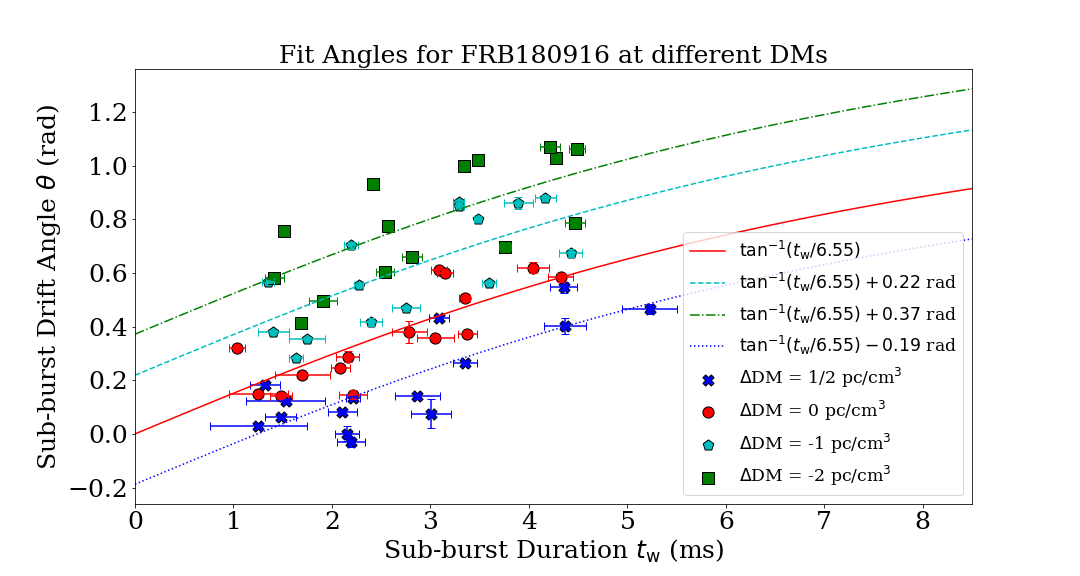
\includegraphics[width=1\textwidth]{B:/dev/sadtrombone/universal/angleatdifferentDMs}
\par\end{centering}
\caption{\label{fig:Angle-at-different}Robustness test: the fit angle $\theta$
vs. sub-burst duration $t_{\mathrm{w}}$ from bursts dedispersed to
small variations in the DM for the source FRB\textasciitilde 180916.
Red points are bursts at $\Delta\mathrm{DM}=0$ which corresponds
to a DM of 348.82 pc/cm$^{3}$. Blue, cyan, and green points are bursts
de-dispersed to $\Delta\mathrm{DM}=0.5,$-1, and -2 pc/cm$^{3}$,
respectively. The red line is fit to the red points and is of the
form $\arctan(t_{\mathrm{w}}/A)$ derived from the dynamical model
described in the main text. Blue, cyan, and green lines are fits found
by adding a rotation (adding an angle) to the $\Delta\mathrm{DM}=0$
model. This plot demonstrates the rotational effect small variations
in the DM has on dynamic spectra of FRBs.}

\end{figure}
\textbf{How do you optimize DM based on the previous test?}

\textbf{Stampcard}

\bibliographystyle{Science}
\bibliography{scibib}

\end{document}
